\UseRawInputEncoding
\documentclass[a4paper,10pt,oneside]{article}
\usepackage{avs,amsmath,epsfig,times,url,hyperref,balance,float,booktabs,placeins,tikz}
\usetikzlibrary{positioning,arrows.meta}

\newcommand{\preset}[1]{\textit{#1}}

\title{REMORA: Real-time Expressive Motion to Output Routing Audio}
\subtitle{A Martial Arts Staff Instrument Driven by Motion}

\twoauthors
{\authorblock{Timoth\'ee Dravet}{Polytech Marseille, Aix-Marseille Universit\'e \\ Marseille, France \\ \email{timothee.dravet@etu.univ-amu.fr}}}
{\authorblock{Daniel Overholt}{CREATE, Aalborg University \\ Aalborg, Denmark \\ \email{dano@create.aau.dk}}}

\begin{document}
\ninept
\maketitle

\begin{sloppy}

\begin{abstract}
REMORA turns a b\^o, the long staff used in martial arts, into a musical instrument:
spins, tilts, and strikes become sound in real time. The instrument is built in two
parts: a small wireless sensor unit rides on the staff and continuously reads its
physical motion, while a companion audio plugin turns that motion into pitch, texture,
and timbre across three very different synthesis voices, from a warm additive choir to a
breath-driven vocal tract. Rather than one fixed gesture-to-sound behaviour, every
mapping from physical motion to sound parameters is a small patch of connected building
blocks - motion sources, shaping math, and synthesis sinks - wired on a visual canvas
inside the plugin, in the spirit of a modular synthesiser's patch cables. The same small
vocabulary of building blocks stretches from a beginner's direct tilt-controlled pitch to
a compound, deliberately one-to-many mapping whose timbre quietly re-randomises itself
with every completed spin, so that no two passes through the same gesture sound quite
identical. Nine such presets currently ship, pared down over the course of development
from a larger, more repetitive set of fifteen.
\end{abstract}

\section{Introduction}
\label{sec:intro}

REMORA grew out of the first author's parallel practice in martial arts and music. The
b\^o itself is a form largely absent from new interfaces for musical expression: a
full-body, two-handed, swung staff with its own weight, reach, and rotational inertia,
quite unlike the small handheld or body-worn sensors most inertial digital instruments
use. Where a martial artist reads speed, force, and reach off the staff by feel, REMORA
reads the same qualities electronically and turns them into sound: a spin becomes a
filter sweep, a slow controlled turn sounds
nothing like a fast, loose one. The instrument's vocabulary is, in that sense, borrowed
directly from the performer's own body of practice rather than invented for the
occasion. Crucially, that vocabulary is not baked into compiled code either: every
motion-to-sound relationship lives inside the plugin as a small, rewireable patch, so
extending or retuning it is an editing operation the performer or instrument-builder can
perform on the same canvas used to play the instrument, rather than a recompile.

Rod-, staff-, and baton-shaped controllers already form a small, recurring family in
this space: the T-Stick's touch-sensitive shaft~\cite{malloch2007tstick}, the Digital
Baton's conducting gesture~\cite{marrin1997digitalbaton}, and Nam's swung Musical
Poi~\cite{nam2013mpoi} among them. What REMORA adds to that family is less a new sensor
than a new relationship: a martial artist's years of staff-handling skill, carried
straight onto a stage as a musical vocabulary. The remainder of this paper describes how
that relationship is built, from the sensor unit on the staff (\S\ref{sec:system})
through the motion-to-sound mapping layer (\S\ref{sec:mapping}) to the resulting catalog
of presets (\S\ref{sec:presets}).

\section{System Design}
\label{sec:system}

\begin{figure}[H]
\centering
\begin{minipage}[c]{0.4\linewidth}
  \centering
  
\includegraphics[width=\linewidth]{Assets/openscad_casing.png}
  \centerline{(a)}
\end{minipage}
\hspace{4mm}
\hfill
\begin{minipage}[c]{0.4\linewidth}
  \centering
  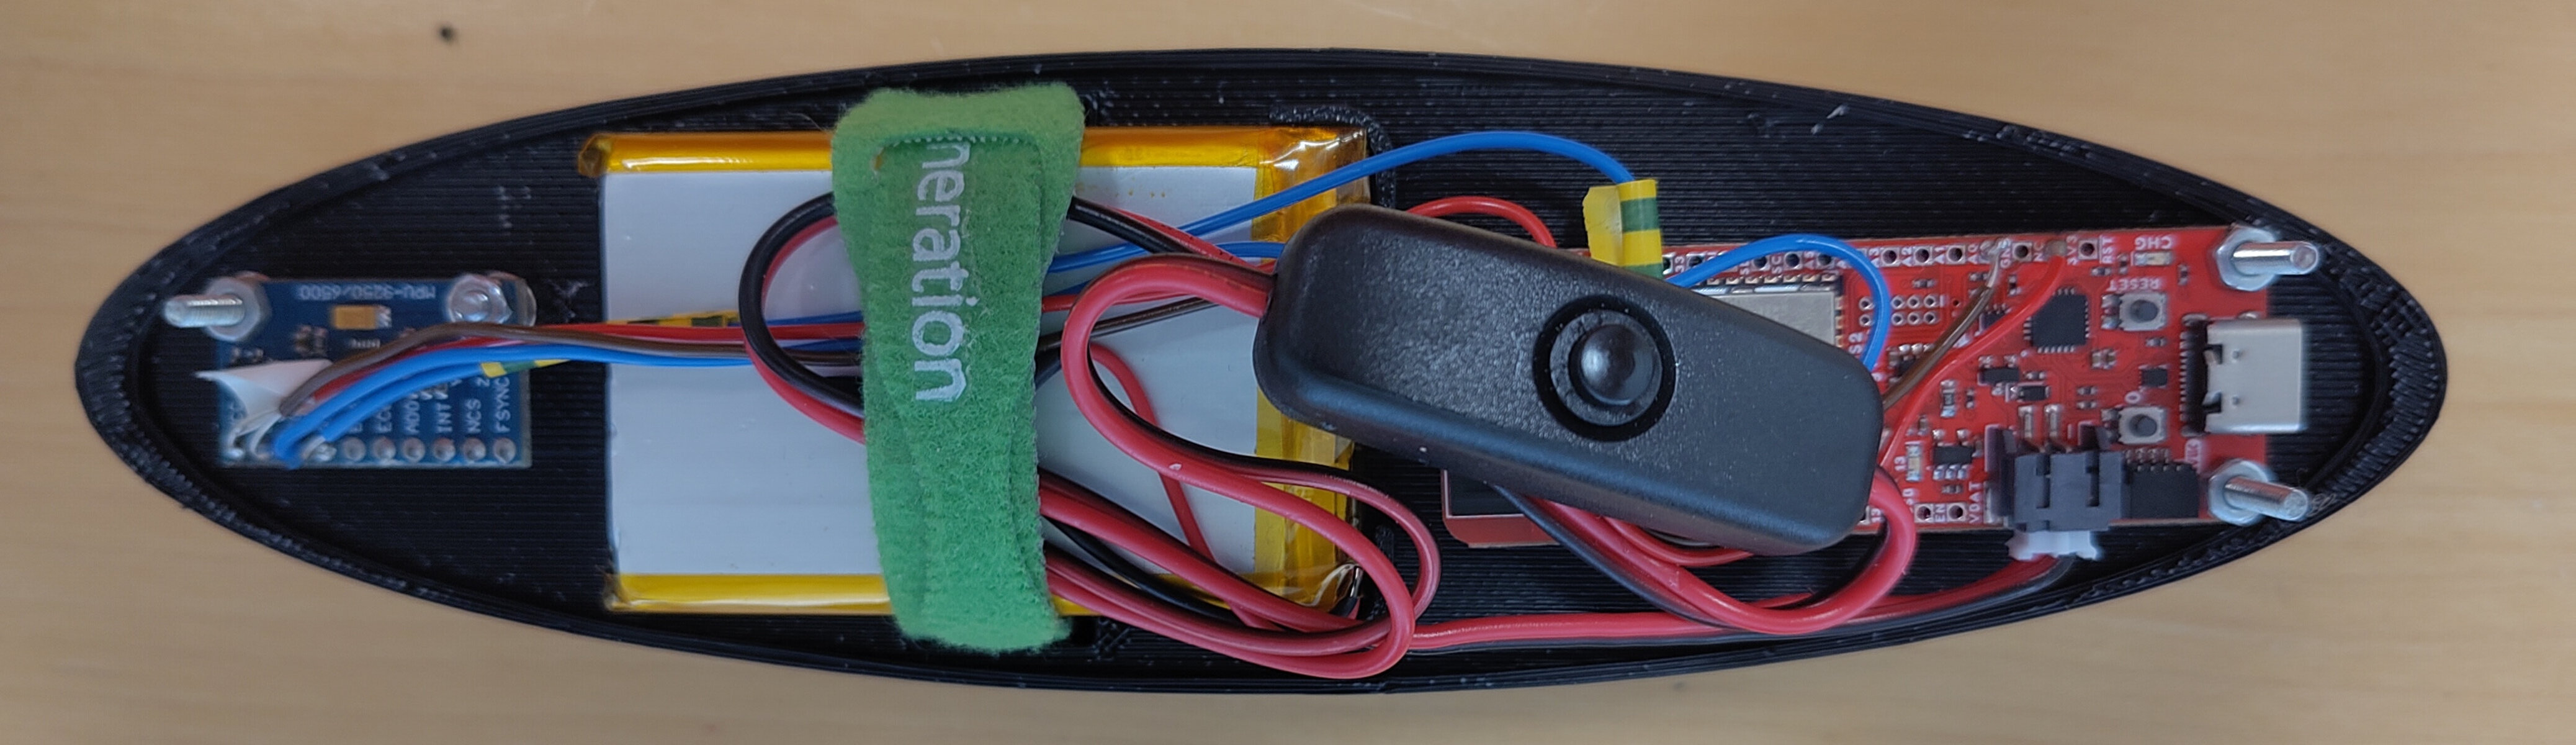
\includegraphics[width=\linewidth]{Assets/hardware_wiring_horizontal.jpg}
  \centerline{(b)}\\[1mm]
  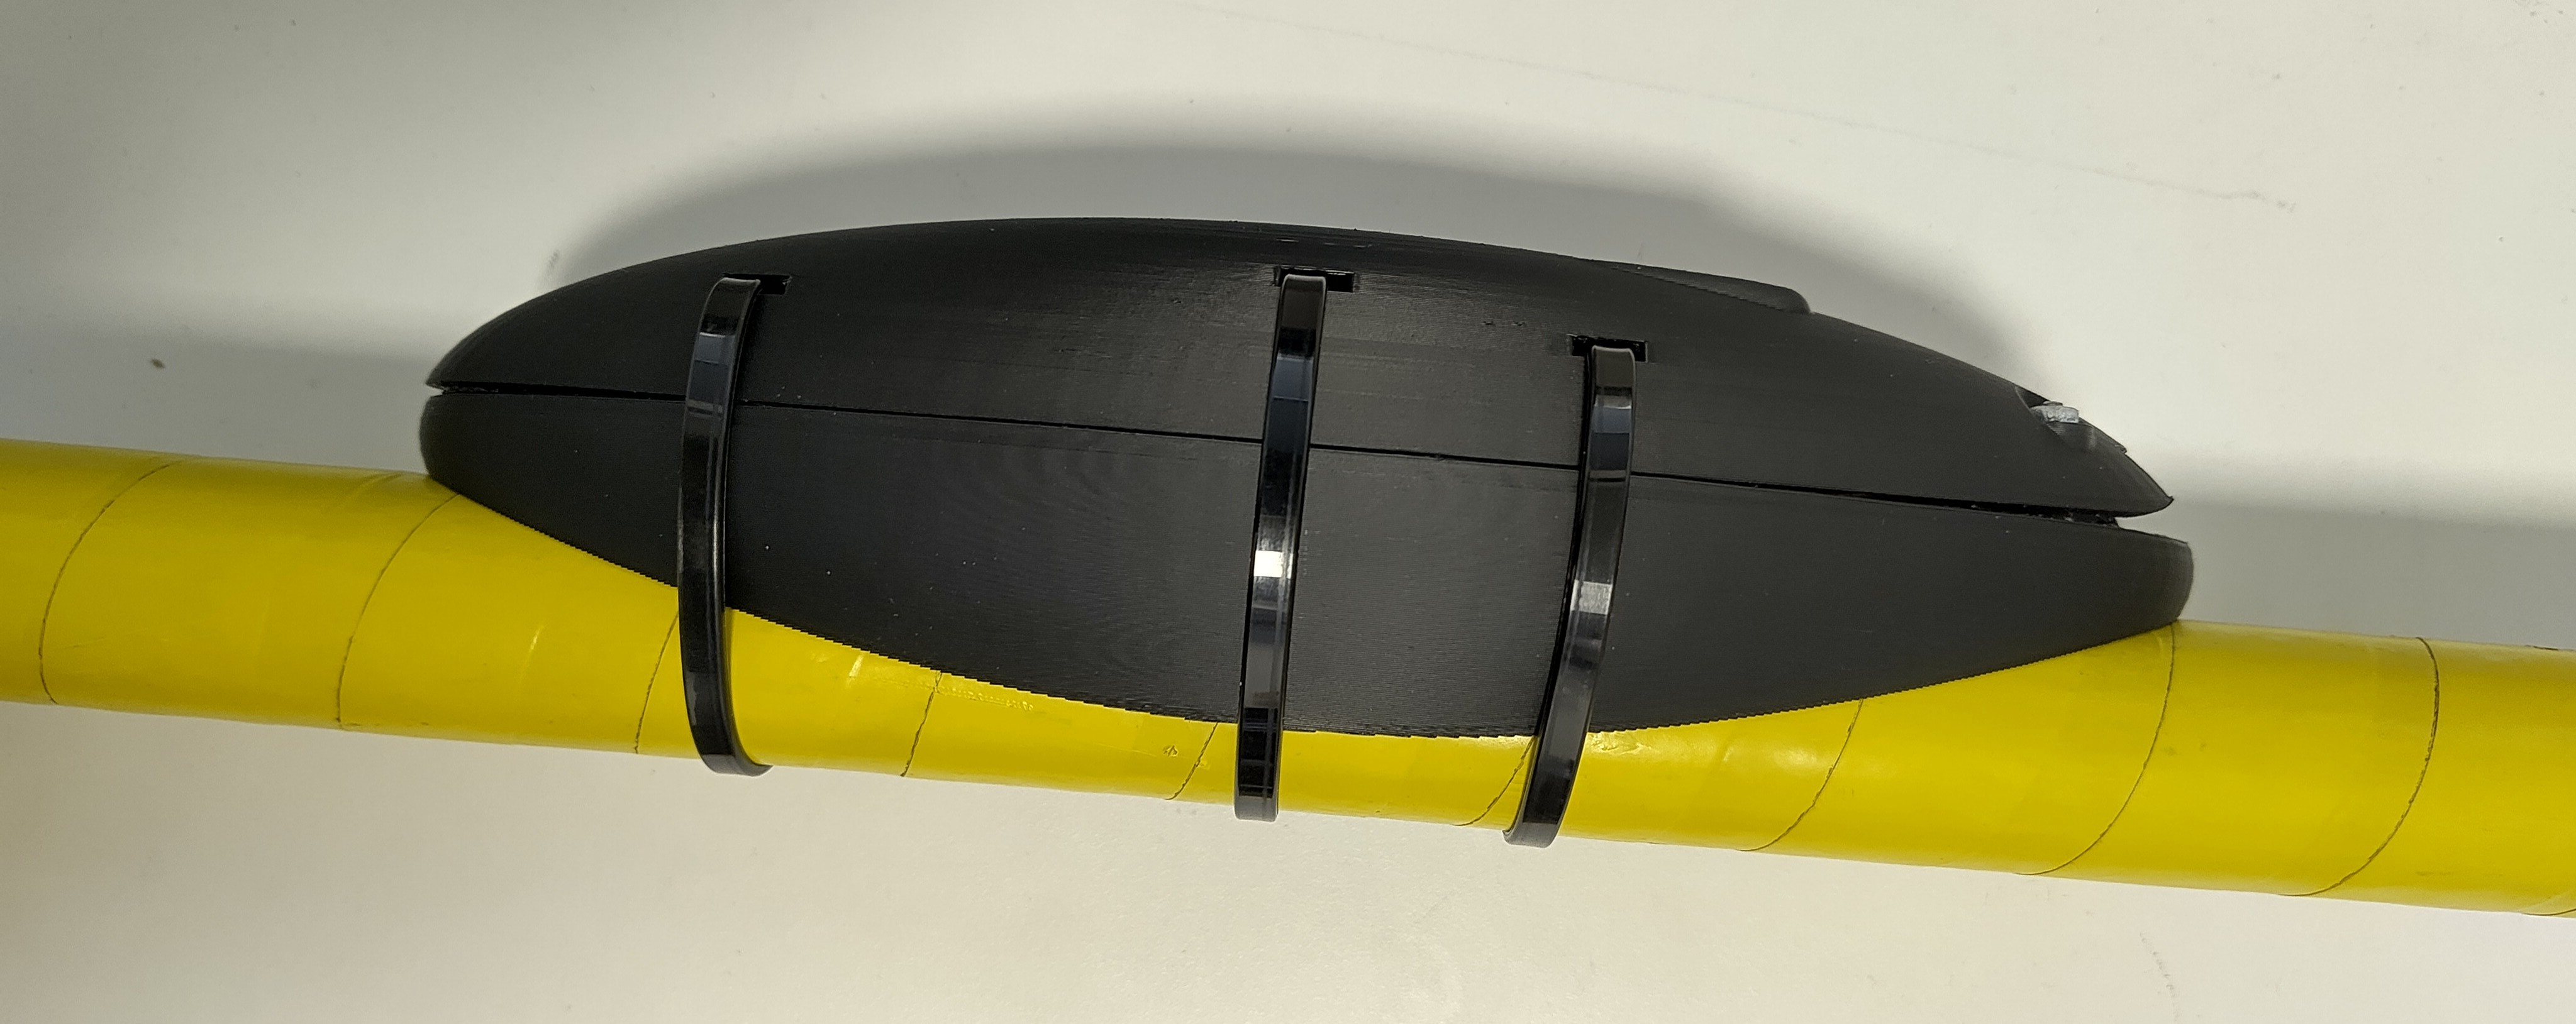
\includegraphics[width=\linewidth]{Assets/casing_horizontal.jpg}
  \centerline{(c)}
\end{minipage}
\caption{The staff-mounted sensor unit, held on with zip ties so it can be repositioned
or removed without marking the staff: (a) the parametric OpenSCAD design; (b) the harware wiring; (c) the
printed enclosure zip-tied to the b\^o.}
\label{fig:enclosure}
\end{figure}

\begin{figure}[H]
\centering
\resizebox{\linewidth}{!}{%
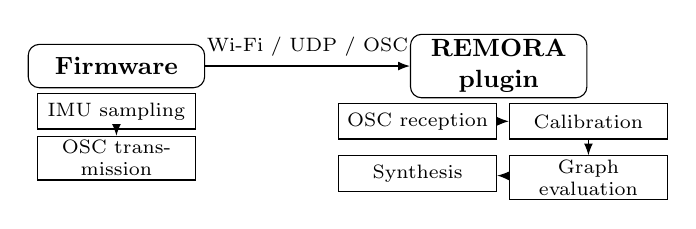
\begin{tikzpicture}[
  box/.style={draw, rounded corners, align=center, text width=2.1cm, minimum height=0.55cm,
    font=\small\bfseries, inner sep=2pt},
  sub/.style={draw, align=center, text width=1.9cm, minimum height=0.45cm, font=\scriptsize,
    inner sep=1.5pt},
  arr/.style={-{Latex[length=1.5mm]}}
]
\node[box] (staff) {Firmware};
\node[sub, below=0.6mm of staff] (collect) {IMU sampling};
\node[sub, below=0.8mm of collect] (send) {OSC transmission};
\draw[arr] (collect) -- (send);

\node[box, right=26mm of staff] (host) {REMORA plugin};
\draw[arr] (staff) -- (host)
  node[midway, above, font=\scriptsize, align=center] {Wi-Fi / UDP / OSC};

\node[sub, below=0.6mm of host, xshift=-1.03cm] (recv) {OSC reception};
\node[sub, right=1.5mm of recv] (calib) {Calibration};
\draw[arr] (recv) -- (calib);
\node[sub, below=2mm of calib] (graph) {Graph evaluation};
\node[sub, below=2mm of recv] (synth) {Synthesis};
\draw[arr] (calib) -- (graph);
\draw[arr] (graph) -- (synth);
\end{tikzpicture}%
}
\caption{Signal path from staff motion to sound: the sensor unit streams orientation
  and inertial data over Wi-Fi to the plugin, which calibrates, derives motion
  qualities, and routes them through a performer-authored patch into one of three
  synthesis engines.}
\label{fig:architecture}
\end{figure}
\FloatBarrier

\subsection{Hardware}
\label{ssec:hardware}

Inside the enclosure shown in Figure~\ref{fig:enclosure}, a SparkFun ESP32-S2 Thing Plus
microcontroller reads a nine-degrees-of-freedom MPU-9250 inertial sensor over I2C and
packs orientation, acceleration, and gyroscope readings into an OSC packet, sent over
UDP at 100~Hz across the microcontroller's own connection to the host computer's Wi-Fi
hotspot. Joining the host's own hotspot rather than a dedicated access point keeps
pairing to a single step, at the cost of a Wi-Fi network name, password, and destination
address that are presently compiled into the firmware rather than set at runtime. Nothing
tethers the performer to a fixed point on stage; a cable is needed only to charge the
unit between sets.

\subsection{Calibration}
\label{ssec:calibration}

Because the sensor can be glued to the staff at any angle (exact placement is never
perfectly reproducible by hand, and often changes from one build of the enclosure to
the next), the plugin calibrates itself the first time the staff is held through three
reference poses. All three poses together fix which physical axis is functioning as
``forward'': the plugin scores every candidate axis by how close to mutually orthogonal
its direction turns out across the three poses, and keeps whichever axis comes closest.
The first two poses then resolve any leftover twist around that axis, by solving for the
small rotation that best lines up the measured forward/up directions with the
instrument's own ideal frame. From then on, the same instrument logic runs correctly no
matter where on the staff the sensor happens to sit, so a performer can move it without
re-learning the instrument underneath.

\subsection{Connection Robustness}
\label{ssec:robustness}

Two recent changes tightened the path from a sensor packet to audible sound. First, the
plugin now treats the incoming stream as stale after 150~ms without a fresh packet,
rather than the previous 500~ms, so a real Wi-Fi dropout is caught and muted noticeably
sooner. Second, that mute no longer shares a single ramp with normal playing: losing the
signal now fades the master gain out over 120~ms (long enough to avoid an audible click)
while recovering it fades back in over a much shorter 10~ms, so the instrument goes
quiet gracefully on dropout but comes back almost immediately once the connection
returns.

\section{Mapping Design}
\label{sec:mapping}

\subsection{Motion Qualities}
\label{ssec:qualities}

Every packet from the sensor is read against a moving reference: not just where the
staff is, but how it got there. Four continuous qualities borrowed from Laban Movement
Analysis are extracted from the motion stream every audio block. How forcefully the
staff moves becomes Weight, read from a leaky integral of its acceleration once gravity
is subtracted out, and typically driving loudness or waveshaping. How suddenly a spin
speeds up or stops becomes Time, driving attack speed and how quickly a chord change
lands. Whether the staff keeps spinning around the same axis or wanders becomes Space, a
timbral focus that tightens or loosens a filter or a chorus spread. How bound or free
the motion is becomes Flow, crossfading between a controlled and a freer, noisier
version of the same sound. Tilt and roll bend pitch and blend voices continuously; a
spin's lap count sweeps a filter cutoff along a slow curve; a stab or strike, a sharp
reversal in the staff-tip's acceleration, triggers a transient, a chord change, or a
percussive burst.

\subsection{Visual Patching}
\label{ssec:patching}

None of the relationships described above is a single fixed algorithm baked into
compiled code. Every one of them is authored as a small patch of connected building
blocks inside the plugin, on a visual canvas in the lineage of
Max~\cite{puckette1988patcher} and Pure Data~\cite{puckette1996puredata}, closer in feel
to the boxes-and-cables idiom that community modular-synthesis software such as VCV
Rack~\cite{belt2017vcvrack} carries over from hardware Eurorack patching than to a
conventional plugin's fixed control panel. Three functional kinds of node populate that
canvas: \emph{sources} (the raw sensor axes and the derived Laban qualities above),
\emph{math} (arithmetic; shaping curves such as range-mapping, logarithmic range-mapping,
clamping, crossfading, and scale-quantizing; lookup tables; and a handful of stateful
primitives - one-pole smoothers, leaky integrators, derivative detectors, hysteresis
gates, and a pseudo-random sample-and-hold), and \emph{sinks} (the exposed parameters of
whichever synthesis voice the patch is driving). A fourth kind, \emph{display}, carries
no signal of its own: a numeric readout, a level meter, and a scrolling scope can be
dropped inline on any wire purely to watch its live value, without altering the patch. A
patch is a directed graph with no cycles
allowed: the plugin topologically sorts it once whenever a wire changes, then re-walks
that fixed order once per audio block, so dragging in a node or dropping a new
connection mid-performance never forces the audio thread to replan anything. A named
preset is nothing more than one such graph, serialised to an XML file and reloaded by
name - the same mechanism a performer's own live patch is saved through, so a
custom mapping built during a rehearsal is stored no differently from a factory one.

That shared vocabulary is small enough to describe in full, yet stretches from the
simplest mapping in the catalog to a considerably more elaborate one. \preset{Simple}
is close to the shortest patch the graph can express: the pitch source feeds one
range-mapping node that becomes the root frequency (wired straight into the additive
voice's sink), and the roll source feeds an absolute-value node into a second
range-mapping node that becomes the gain (wired into its own, separate gain sink) - two
motion sources and three math nodes feeding two sink nodes in total, wired once and left
alone for the rest of the performance. \preset{Azimut Kinetic} sits at the other end of
the same vocabulary. Its
pitch and gain follow the same lookup-table-driven facing logic as the rest of the
Azimut family, but its timbre is deliberately one-to-many~\cite{hunt2002mapping}: a
single smoothed rotation-speed value fans out simultaneously into the filter cutoff,
harmonic brightness, waveshaping drive, noise amount, vibrato and tremolo depth, and
reverb send, so a spin sounds progressively buzzier, noisier, and more reverberant the
faster it turns, rather than moving one parameter in isolation. Layered on top of that
energy value, a derivative node watches the continuous spin-lap counter for the instant
each full rotation completes and fires a one-block pulse into a sample-and-hold node,
which then latches four fresh pseudo-random values; each value is chased by its own slow
one-pole ``drift channel'' - closing roughly 5\% of the remaining distance to its new
random target on every audio block, so the drift glides rather than jumps - and folded
back, in a small proportion, onto the cutoff, drive, noise amount, and harmonic
brightness the energy value already set.
The result is a mapping that never quite repeats itself: two visually identical spins
land on two different, nearby timbres, because every completed rotation quietly
re-rolls where the tone drifts to next - an instability the graph's existing math nodes
are enough to build, with no bespoke code and no audio-thread cost beyond four extra
smoothers.

\begin{figure}[t]
  \centering
  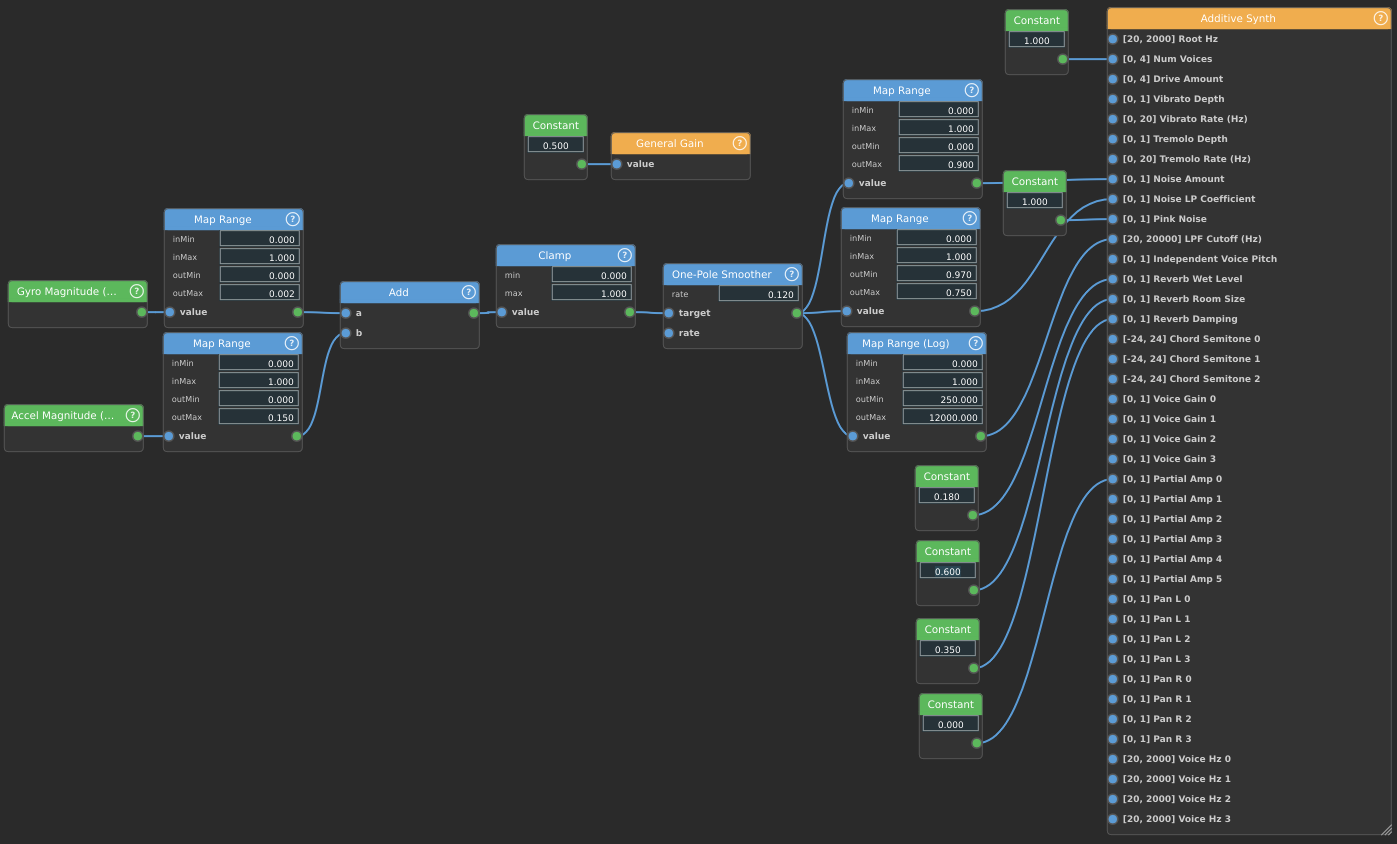
\includegraphics[width=\linewidth]{Assets/preset.png}
  \caption{The \preset{Wind Noise} preset, seen inside the plugin: motion sources
  (green) - gyroscope and accelerometer magnitude - run through shaping and smoothing
  math (blue) into the exposed parameters of the additive-synthesis voice (orange).
  There is no pitch input anywhere in this patch: only motion energy, shaping noise
  amount and the master filter cutoff.}
  \label{fig:preset}
\end{figure}
\FloatBarrier

\subsection{Synthesis Engines}
\label{ssec:engines}

What a patch's output actually sounds like depends on which of three synthesis voices
its sink nodes are wired into. A default additive engine sums four voices of six
phase-locked harmonics each, vibrato- and chorus-detuned into a warm, faintly unstable
choir that a mapping can drive into a rasping saturation or filter down to a single dark
hum; a short comb resonator gives every voice a string-like colouration. That same engine
also carries its own built-in noise generator and filter, and it is this path, not a
separate voice, that \preset{Wind Noise} actually drives (Figure~\ref{fig:preset}): the
patch wires nothing at all into the engine's pitch inputs, only motion-energy-shaped
noise and filter cutoff, for a windy, textural character with no fixed pitch centre at
all. A second, granular engine sits alongside the additive one, synthesising its own
two-second bed of shifting harmonics and filtered noise and scattering up to 64
overlapping grains across it (forward, backward, panned, re-pitched); it is fully
implemented but not yet wired into any preset in the current catalog, so it stays silent
until a future patch calls on it. A third engine ports Neil Thapen's \emph{Pink
Trombone}~\cite{thapen2017pinktrombone}, a digital-waveguide vocal tract excited by a
glottal-pulse model and breathed into with filtered noise, so the instrument can also
simply speak, or half-speak, rather than only sing - the one engine with a preset built
specifically around it, \preset{Vocal Tract}. An engine a patch never wires into is
skipped entirely for that block, so presets built on one voice never pay for the other
two.

\section{Preset Vocabulary}
\label{sec:presets}

Nine named presets currently ship with the instrument (Table~\ref{tab:presets}), graded
by the physical vocabulary they ask of a performer rather than uniform in difficulty.
\preset{Simple} asks only for basic tilt and roll, an easy way in that needs no martial
background at all. The \preset{Azimut} and \preset{Martial} families reward the
staff-handling skill a martial artist already carries onto a stage: they derive a facing
direction and a spin quality straight from the calibrated motion stream, without ever
touching a magnetometer (which a stage rig's own electronics would only confuse), so
that where the staff points and how it turns becomes part of the music. \preset{Wind
Noise} trades pitch for a breathy, filtered-noise texture sustained by nothing but
motion; \preset{Vocal Tract} pushes the same sensor stream into something closer to a
voice than a synthesiser. Each preset is less a separate program than a different
character the same instrument can take on, chosen for a set the way a performer chooses
which piece to play next, rather than a fixed, single-piece score.

\begin{table}[t]
\centering
\small
\begin{tabular}{@{}p{0.32\linewidth}p{0.58\linewidth}@{}}
\toprule
Preset & Character \\
\midrule
\preset{Simple} & Pitch from tilt, volume from roll; one plain sine voice. \\
\preset{Wind Noise} & No pitch; motion energy swells filtered noise into gusts. \\
\preset{Bowed Chord} & Chromatic root from pitch; yaw/roll pick the chord; spin speed drives it like bow pressure. \\
\preset{Lead + Drone} & Major-scale lead over a 4-voice drone; yaw crossfades two drone voices. \\
\preset{Martial Momentum} & Root from spin plane/direction; glide speed set by spin momentum. \\
\preset{Azimut Kinetic} & Facing-based root; a single rotation-speed value drives filter, drive, noise, and reverb at once, with per-rotation stochastic drift. \\
\preset{Speed Gate} & Slow: pentatonic melody. Fast: crossfades into the Azimut facing/spin-based root and filter mapping. \\
\preset{Spin Voices (Scale)} & Roll picks 1 of 4 scale-quantized voices; the rest hold their last pitch/gain. \\
\preset{Vocal Tract} & Physically-modeled voice; pitch/roll/yaw shape glottal pitch and vowel; jabs add consonant-like bursts. \\
\bottomrule
\end{tabular}
\caption{The nine presets currently shipping, in load order.}
\label{tab:presets}
\end{table}
\FloatBarrier

This catalog is smaller than it once was. Fifteen mappings were implemented over the
course of development, but several turned out to be near-duplicates of one another once
built - a plain spin-driven pentatonic melody and its Laban-shifted cousin, three
separate Azimut variants that each added one extra timbral trick (a spin-count filter
sweep, a speed-tracking filter, a motion-driven reverb) on top of an otherwise identical
mapping. Rather than ship all fifteen, the list was pruned to nine: \preset{Azimut
Kinetic} folds every one of those three Azimut timbral tricks into a single one-to-many
mapping (\S\ref{sec:mapping}) instead of shipping them as separate, thinner presets, and
similar consolidations retired the redundant spin- and momentum-only mappings. The six
retired mappings still exist as graphs in the source tree - useful engineering reference
points and starting patches to fork from - but are no longer surfaced in the plugin's
own preset selector.

\section{Evaluation}
\label{sec:evaluation}

Ten performers with no prior exposure to REMORA (N=10) tried the instrument in a short,
informal pilot session: each was calibrated (\S\ref{ssec:calibration}), given a brief
demonstration, then played freely across a subset of the nine presets before completing
a short questionnaire. Their backgrounds were, by design, uneven: self-rated
martial-arts or staff-handling experience skewed low (nine of ten at 1 or 2 out of 5),
general music experience moderate, and prior experience with motion-controlled
instruments mixed - a pool weighted toward newcomers to the staff form itself, the
audience \preset{Simple} was designed to admit (\S\ref{sec:presets}).

Six statements about the playing experience, each rated on a five-point scale, are
summarised in Table~\ref{tab:eval}. Comfort scored highest and most consistently: the
enclosure and staff form factor did not get in the way of play. Novelty and absorption in
the music rather than the mechanics followed closely, suggesting the
motion-to-sound vocabulary reads as expressive enough to disappear behind, even in a
short first session. Predictability of the mapping and felt expressiveness scored lower
and more variably, consistent with the free-text feedback below: several participants
could point to specific gestures whose effect on the sound they could not reliably
predict.

\begin{table}[H]
\centering
\small
\begin{tabular}{@{}lc@{}}
\toprule
Statement & Mean (SD) \\
\midrule
Predictability & 3.4 (1.2) \\
Comfort & 4.0 (1.0) \\
Novelty & 3.9 (0.9) \\
Expressiveness & 3.3 (1.2) \\
Absorption & 3.9 (0.9) \\
Musical satisfaction & 3.6 (1.3) \\
\bottomrule
\end{tabular}
\caption{Mean (SD) agreement, 1--5 scale, N=10, on six playing-experience statements from
the post-session questionnaire.}
\label{tab:eval}
\end{table}
\FloatBarrier

Preference across presets split unevenly rather than converging on one: \preset{Azimut
Kinetic} was the most-picked (3/10), followed by \preset{Wind Noise} and \preset{Lead +
Drone} (2/10 each), with \preset{Spin Voices} and \preset{Vocal Tract} picked once each and
one participant declining to single one out (``all of them are great''). The reasons given
tracked each preset's intended character: \preset{Azimut Kinetic} for matching lived
martial-arts habit (``It matches best what I know from my martial art experience''),
\preset{Wind Noise} for needing no music or martial background at all (``just pure
instinct and simple movements''), \preset{Lead + Drone} for being the easiest to steer a
melody with while still sounding grounded.

The clearest actionable finding was not something we asked about directly. Three of ten
participants raised the same limitation unprompted, in three different free-text answers:
a striking or thrusting motion that felt physically decisive registered no equivalent
change in the sound (``Occasional frustration when a movement that felt impactful had no
impact on the sound''; ``The thrust are not well detected''; ``Add \emph{thrust} detection
support or fix the existing''). None of the nine shipping presets currently derives a
dedicated signal from a stab or strike beyond the generic transient described in
\S\ref{ssec:qualities}, so this is a concrete, convergent request for a motion quality the
mapping vocabulary does not yet expose. A second, smaller cluster of feedback concerned the
node-graph editor itself rather than any preset: one participant who otherwise rated the
instrument highly asked for the wiring interface to be made easier, ``maybe some kind of
tutorial'', echoing the same complexity the graph exposes to a performer who only wants to
play, already named as a limitation in \S\ref{sec:discussion}. Reported frustration was
otherwise mostly framed as ordinary friction rather than a reason to stop - ``no, really
easy and when a bit hard it's just a learning experience!'', ``did not make me want to stop
but had to adjust'' - with one exception noting the instrument felt enjoyable to play but
did not, on its own, motivate further practice.

\section{Discussion}
\label{sec:discussion}

Everything described above is grounded in the system as it runs today, exercised
continuously through the first author's own development and rehearsal, and now also in
the pilot session reported in \S\ref{sec:evaluation}: ten first-time players found the
instrument comfortable and absorbing enough to lose themselves in, while converging
independently on the same gap - thrust and strike detection - as the mapping
vocabulary's clearest missing piece. Ten participants is a pilot, not a validated
usability study, and the claims above should be read accordingly.

The instrument also carries limitations worth naming plainly: Wi-Fi pairing is still a
manual, reflash-to-change affair rather than a runtime setting, even after the dropout
handling itself was tightened (\S\ref{sec:system}); yaw drift is bounded to sessions of
tens of minutes by assumption rather than measurement; the single inertial sensor gives
REMORA no sense of a second performer, so it remains a solo instrument for now; and the
node-graph editor, while it is what makes the preset catalog reproducible and extensible
at all, exposes that same complexity to a performer who only wants to pick a preset and
play, with no simplified performance-only view that hides the graph until it is asked
for.

One extension is next on the list regardless of the evaluation's findings above:
replacing the compiled-in Wi-Fi hotspot join with an ESP-NOW peer-to-peer link between
the staff's microcontroller and a second one tethered to the host, which would drop the
SSID, password, and destination IP address currently baked into firmware in favour of
pairing by MAC address, at the cost of one extra piece of hardware in the signal chain.

\section{Conclusion}
\label{sec:conclusion}

REMORA reads a martial artist's own staff-handling vocabulary - spins, tilts, strikes -
directly off a b\^o and turns it into sound, without baking any single gesture-to-sound
behaviour into compiled code: every mapping is instead a small, rewireable patch built
from the same handful of source, math, and sink nodes, stretching from the one-line
\preset{Simple} mapping to the self-varying \preset{Azimut Kinetic} (\S\ref{sec:mapping}).
Nine presets built from that vocabulary currently ship, pruned down from fifteen once
overlapping mappings became apparent (\S\ref{sec:presets}). What this paper has
established is that the instrument works end to end, from a self-calibrating sensor
unit through to three distinct synthesis voices (\S\ref{sec:system}), and that it does
so in hands other than its designer's: a ten-participant pilot (\S\ref{sec:evaluation})
found it comfortable and absorbing to play regardless of prior martial-arts or music
background, while converging on strike detection as the first thing to fix. Confirming
that finding at a larger scale, together with the ESP-NOW rework in
\S\ref{sec:discussion}, is what's next.

\section{Acknowledgment}
\label{sec:ack}

This work was carried out during the first author's internship at CREATE, Aalborg
University, Denmark. Firmware, plugin source, enclosure files, and the current preset
catalog (plus the retired mappings kept as reference graphs, \S\ref{sec:presets}) are
available at \url{https://github.com/TimotheeDvt/REMORA}.

\balance
\bibliographystyle{avs}
\bibliography{references}

\end{sloppy}
\end{document}
